\section{modules.\-hpp \-File \-Reference}
\label{modules_8hpp}\index{modules.\-hpp@{modules.\-hpp}}


\-Convenience header for modules.  


{\ttfamily \#include \char`\"{}modules/battery.\-hpp\char`\"{}}\*
{\ttfamily \#include \char`\"{}modules/digital\-\_\-output.\-hpp\char`\"{}}\*
{\ttfamily \#include \char`\"{}modules/led\-\_\-array.\-hpp\char`\"{}}\*
{\ttfamily \#include \char`\"{}modules/diff\-\_\-drive.\-hpp\char`\"{}}\*
{\ttfamily \#include \char`\"{}modules/sound.\-hpp\char`\"{}}\*
{\ttfamily \#include \char`\"{}modules/acceleration\-\_\-limiter.\-hpp\char`\"{}}\*
\-Include dependency graph for modules.\-hpp\-:
\nopagebreak
\begin{figure}[H]
\begin{center}
\leavevmode
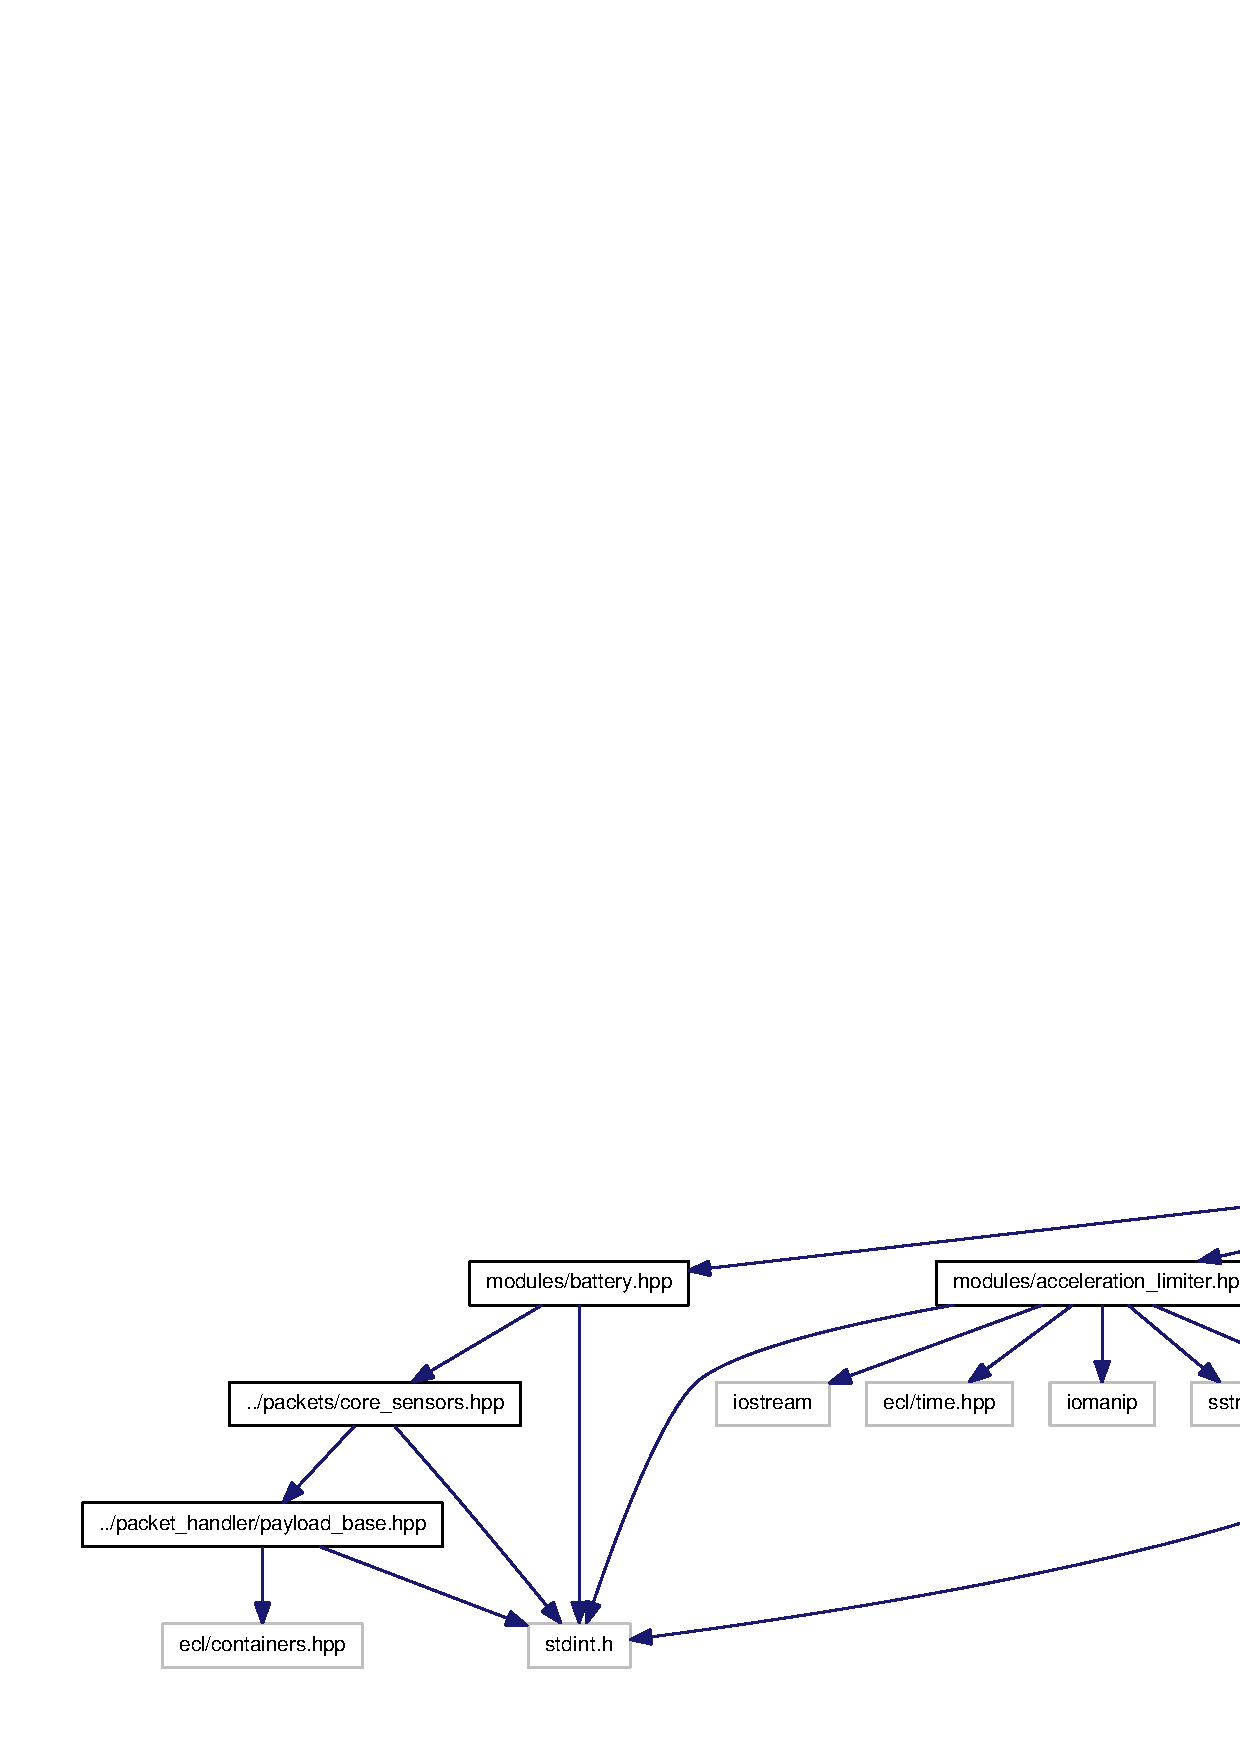
\includegraphics[width=350pt]{modules_8hpp__incl}
\end{center}
\end{figure}
\-This graph shows which files directly or indirectly include this file\-:
\nopagebreak
\begin{figure}[H]
\begin{center}
\leavevmode
\includegraphics[width=350pt]{modules_8hpp__dep__incl}
\end{center}
\end{figure}


\subsection{\-Detailed \-Description}
\-Convenience header for modules. \-License\-: \-B\-S\-D {\tt https\-://raw.\-github.\-com/yujinrobot/kobuki/master/kobuki\-\_\-driver/\-L\-I\-C\-E\-N\-S\-E} 

\-Definition in file {\bf modules.\-hpp}.

